\documentclass[a4paper, oneside, 10pt]{article}
\usepackage[english]{babel}
\usepackage[unicode]{hyperref}
\usepackage[utf8x]{inputenc}
\usepackage{listings}
\usepackage{graphicx}
\usepackage{svg}
\usepackage{tikz}
\usepackage{float}
\usepackage{subcaption}


\graphicspath{{media/}}
\date{\today}
\title{}
\author{Alexandre Adalardo de Oliveira}
\begin{document}




\section{\texorpdfstring{Dados no  dispositivo móvel}{ da Parcela PEIC}}
\label{sec:coleta_de_dados_por_dispositivo_movel}


\href{https://opendatakit.org/}{Open Data Kit} é um projeto colaborativo de código aberto para coleta, armazenamento e gerenciamento de dados. A proposta é disponibilizar instrumentação de baixo custo para coleta de dados que possa ser utilizada em áreas remotas e sem infraestrutura de internet. Permite a coleta de dados tanto online quanto offline e tem a possibilidade de descarregar dados quando se conecta a rede.

Desenvolvemos um formulário baseado nessa plataforma para fazer o censo da Parcela Permanente da Ilha do Cardoso e também para a checagem de dados. O formulário atual é apenas para obter informações das árvores baseadas no último censo que se iniciou em 2019.

Para utilizá-lo é preciso instalar o \textbf{ODKCollect} através da \textbf{Play Store} em dispositivo móvel Android, de preferência um tablet, mas um smartphone dá conta do recado.
Depois de instalado é necessário inserir os arquivos dos formulários e dos dados da parcela no dispositivo para ativar o formulário. Os arquivos necessários estão no googe drive:

\href{https://drive.google.com/drive/folders/1fVV25eK96sS1gSvhE8xhcLftTbL6dQI3?usp=sharing}{peicTrees data}
Caso o link acima não funcione entre copie o link abaixo no seu navegador:

\begin{itemize}
  \item  \small\textbf{https://drive.google.com/drive/folders/1fVV25eK96sS1gSvhE8xhcLftTbL6dQI3?usp=sharing}:
\end{itemize}


\subsection{\texorpdfstring{Instalando o formulário PEIC}{Instalando o formulario PEIC}}
\label{sec:instalando_o_formulario_peic}


Vamos usar um formulário chamado \textbf{peicTrees}. Depois de instalar o aplicativo \textbf{ODKCollect} no dispositivo móvel, abra e inicie um novo projeto cadastrando um email.  Uma pasta será criada na memória de \textbf{Armazenamento interno} do sistema android do dispositivo. Na versão 2021.2 do aplicativo \textbf{ODKCollect} os arquivos de formulários bem como os dados estão em um diretório projeto criado pelo usuário em $>Android > data > org.odk.collect.android> files > projects > 'uma pasta do projeto' >$. A pasta dentro do projeto tem as seguintes subpastas:
\begin{itemize}
  \item estrutura de pasta do \textbf{ODKCollect}:

  \begin{enumerate}
      \item instances
      \item forms
      \item metadata
      \item layer
    \end{enumerate}
    \end{itemize}


Para usar o aplicativo vamos precisar colocar os seguintes arquivos e pastas dentro da pasta \textbf{forms}:
  \begin{itemize}
  \item O formulário de entrada de dado:s \textbf{peicTrees.xml}
  \item Uma pasta com as mídia e dados, que precisa ter o nome: \textbf{peicTrees-media}

    Esta pasta de \textit{media} deve conter:

    \begin{itemize}
    \item dados do censo : \textit{dataTrees.csv}
    \item figura com o mapas das árvores por subpacelas de 20 x 20 m (no caso subparcela A00: \textit{mapTrees\_A00.svg}).\\
        São 256 subparcelas, caso seu dispositivo móvel tenha pouca memória disponível, suba apenas as que pretende visitar. 
      \end{itemize}
    \end{itemize}



\section{\texorpdfstring{Usando o formulário peicTrees}{Usando o formulario peicTrees}}
\label{sec:usando_o_formulario_censopeic}


Abra o aplicativo e siga a sequência de eventos e seleções descritas na tela. 

Para avançar entre as páginas do formulário deve-se usar o gesto do indicador da esquerda para a direita.

\subsection{\texorpdfstring{Página inicial}{Pagina inicial}}
\label{sec:pagina_inicial}



\begin{figure}
  \centering
  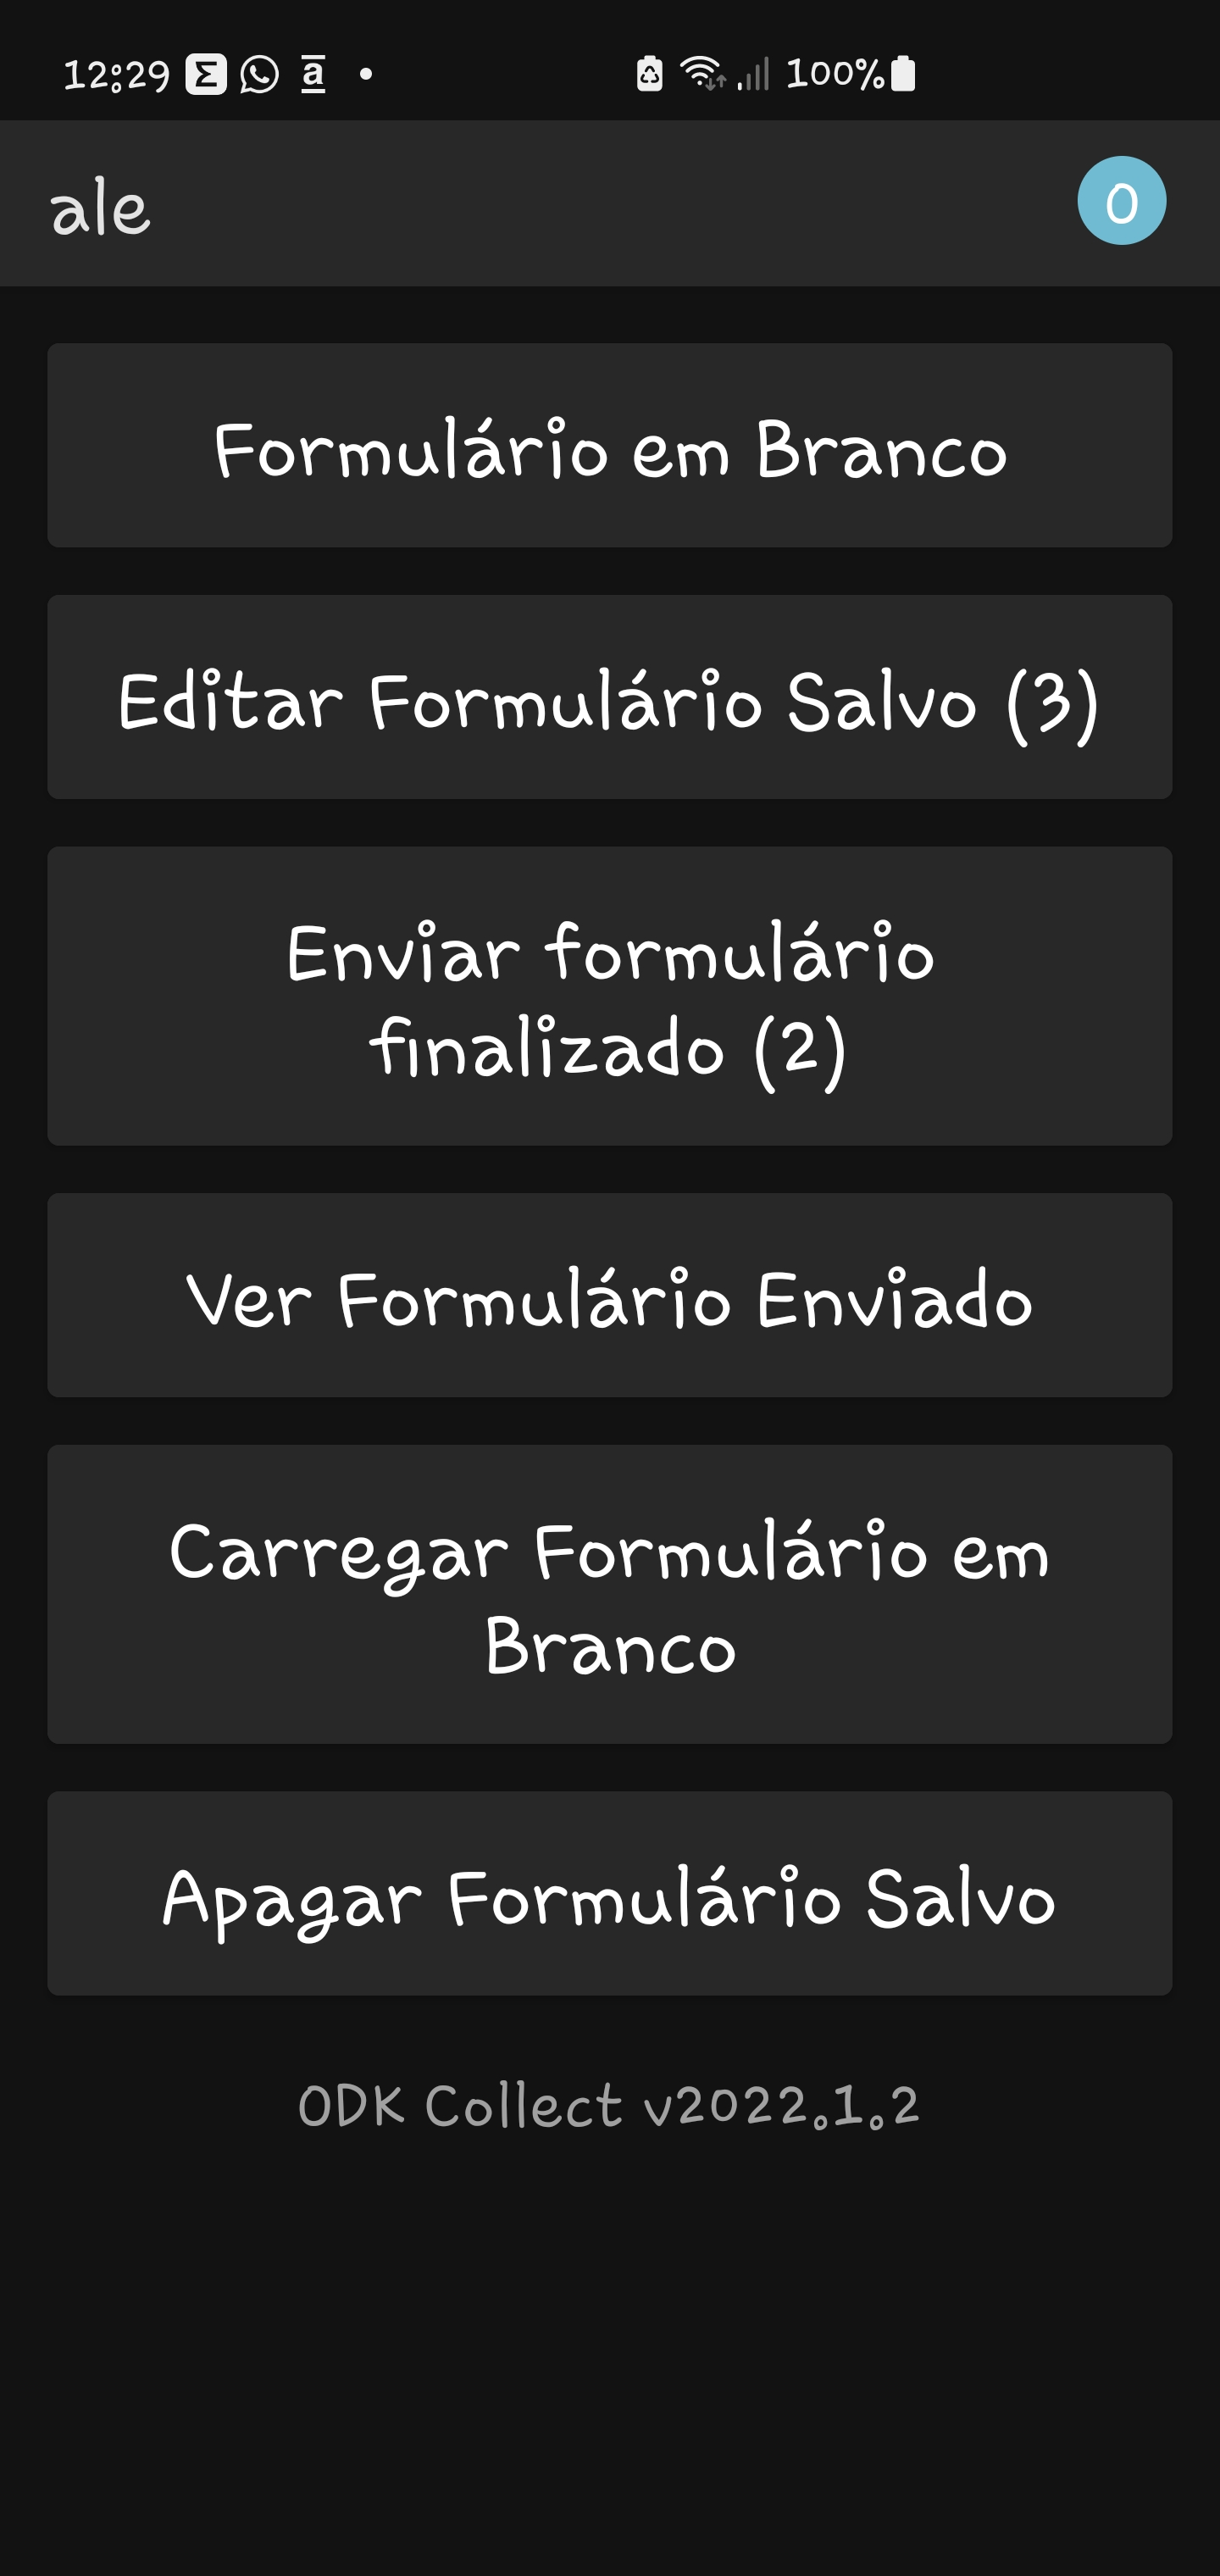
\includegraphics[width=0.5\textwidth]{media/odkSelectBranco.jpg}
  \caption{No \textbf{\emph{\underline{Menu Principal}}} selecione a opção:\textbf{Formulário em Branco}}

\end{figure}



Deve aparecer o nome do formulário xml que foi copiado para o dispositivo. Caso não apareça, houve algum problema , verifique se foi copiado na pasta correta. 


\begin{figure}
  \centering
  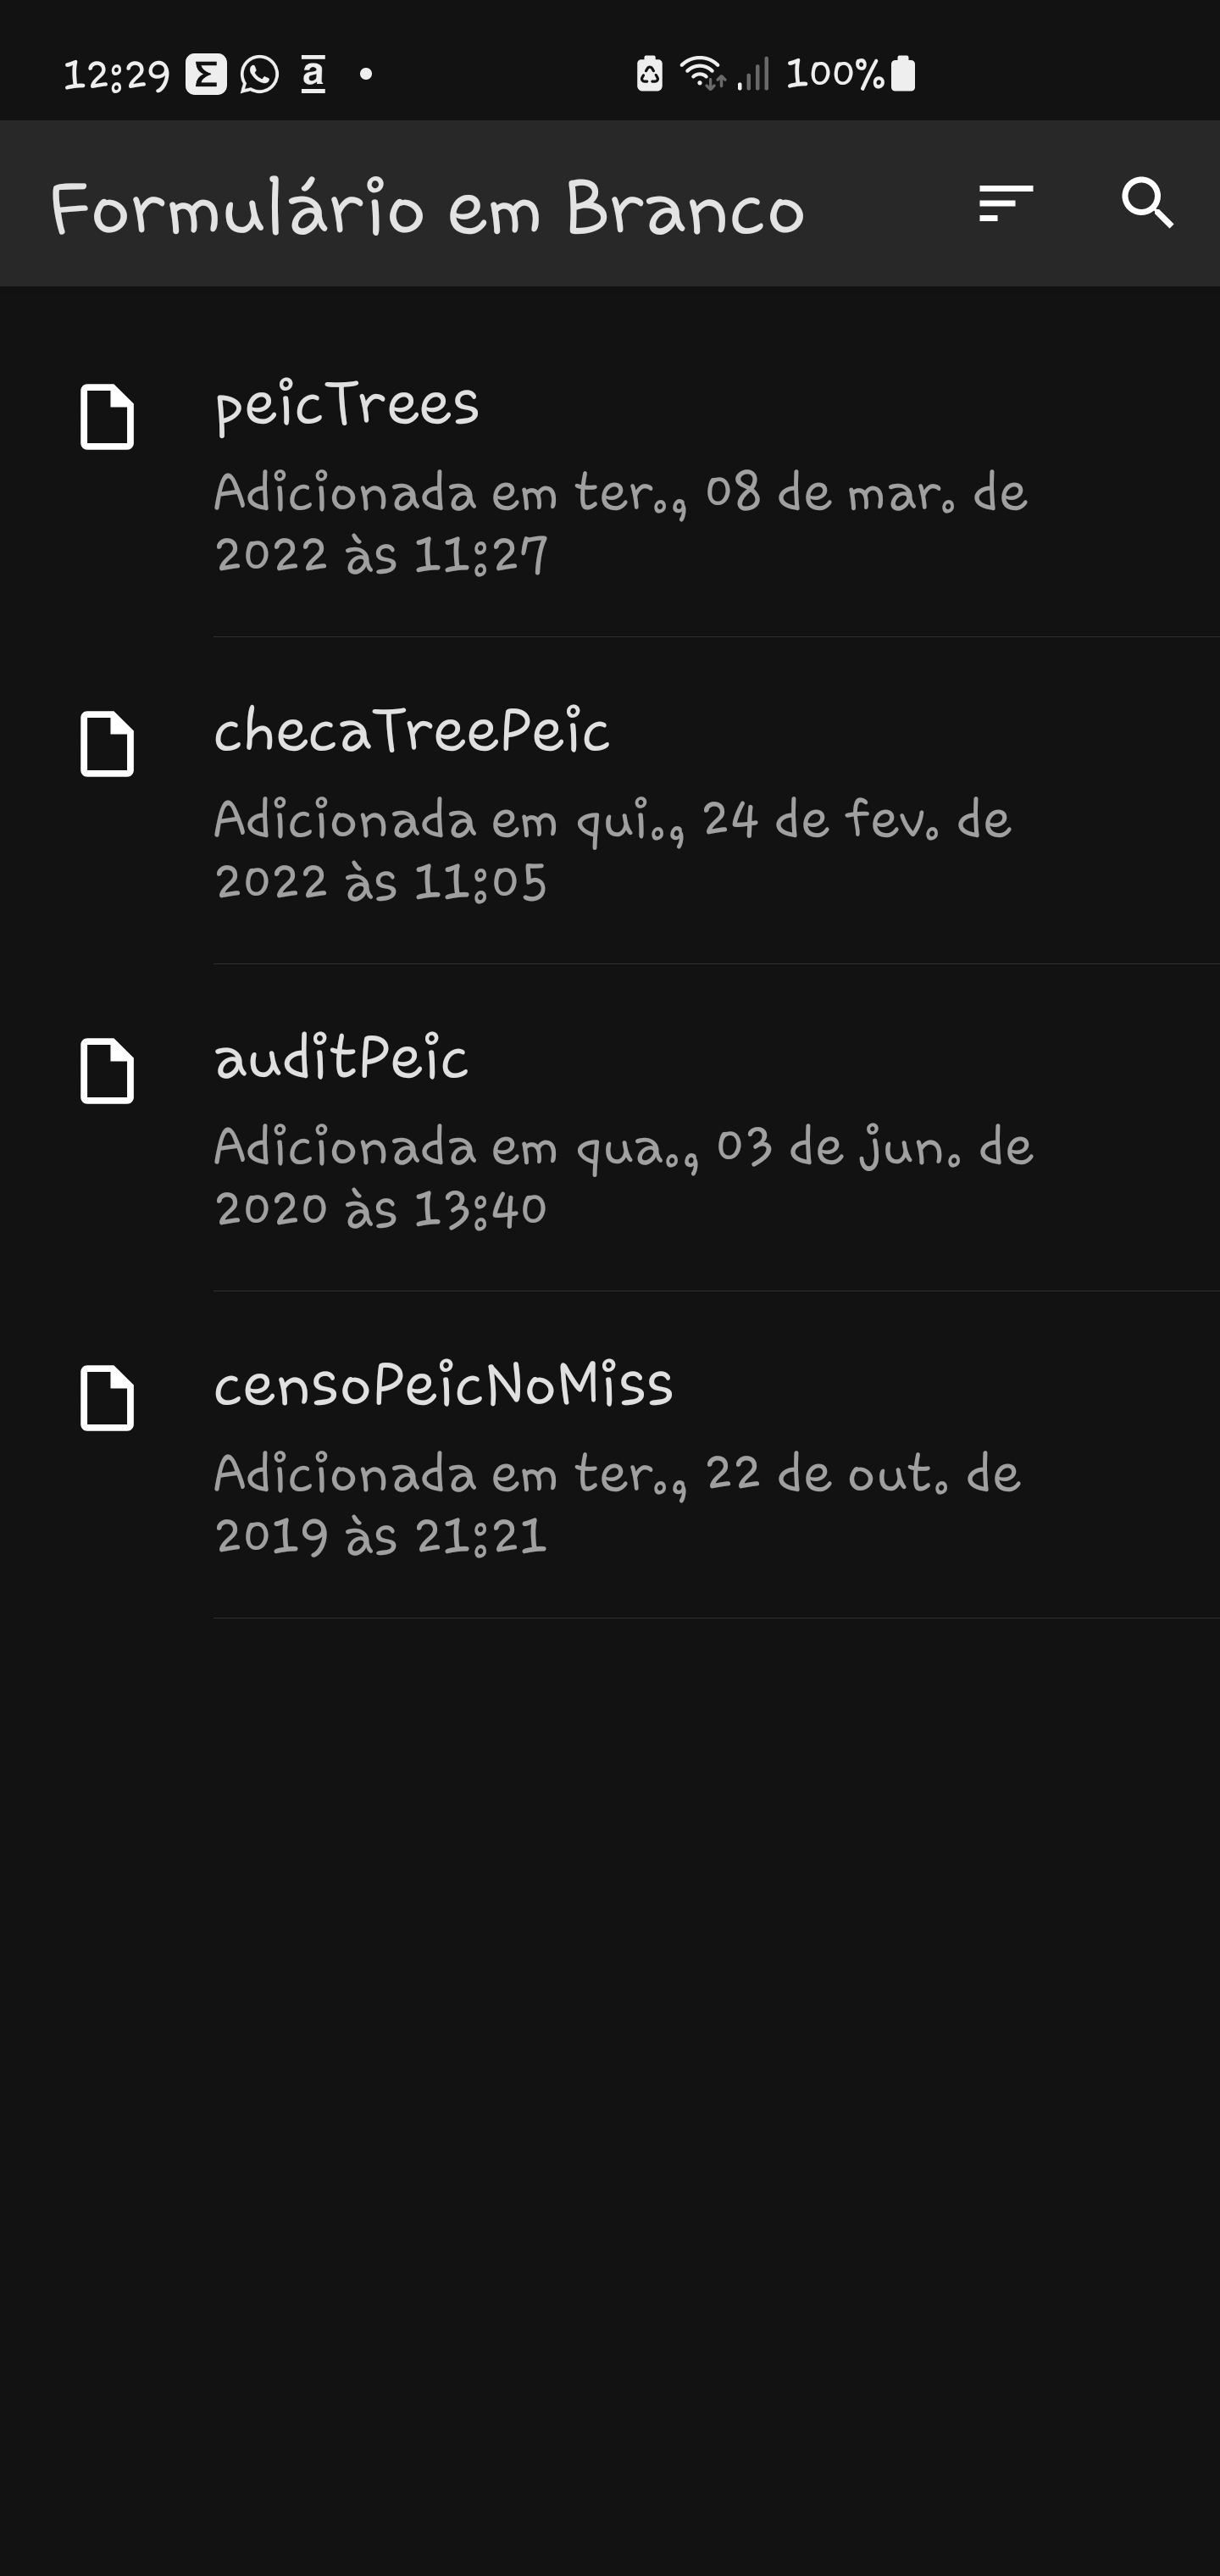
\includegraphics[width=0.5\textwidth]{media/odkSelectForm.jpg}
  \caption{ Selecione a opção:\textbf{peicTrees}. Caso não esteja disponível verifique se os arquivos foram copiados corretamente.}

\end{figure}


\subsection{\texorpdfstring{SubParcela}{SubParcela}}
\label{sec:arvores}


Na primeira tela do aplicativo é preciso selecionar o código da subparcela na qual o usuário quer acessar os dados. Os códigos das subparcelas são compostos de uma letra maíuscula \textbf{A-P} que corresponde a coluna (coordenada x)  e um número com dois dígitos \textbf{00:15} que corresponde as linhas (coordenada y).


\begin{figure}
  \centering
  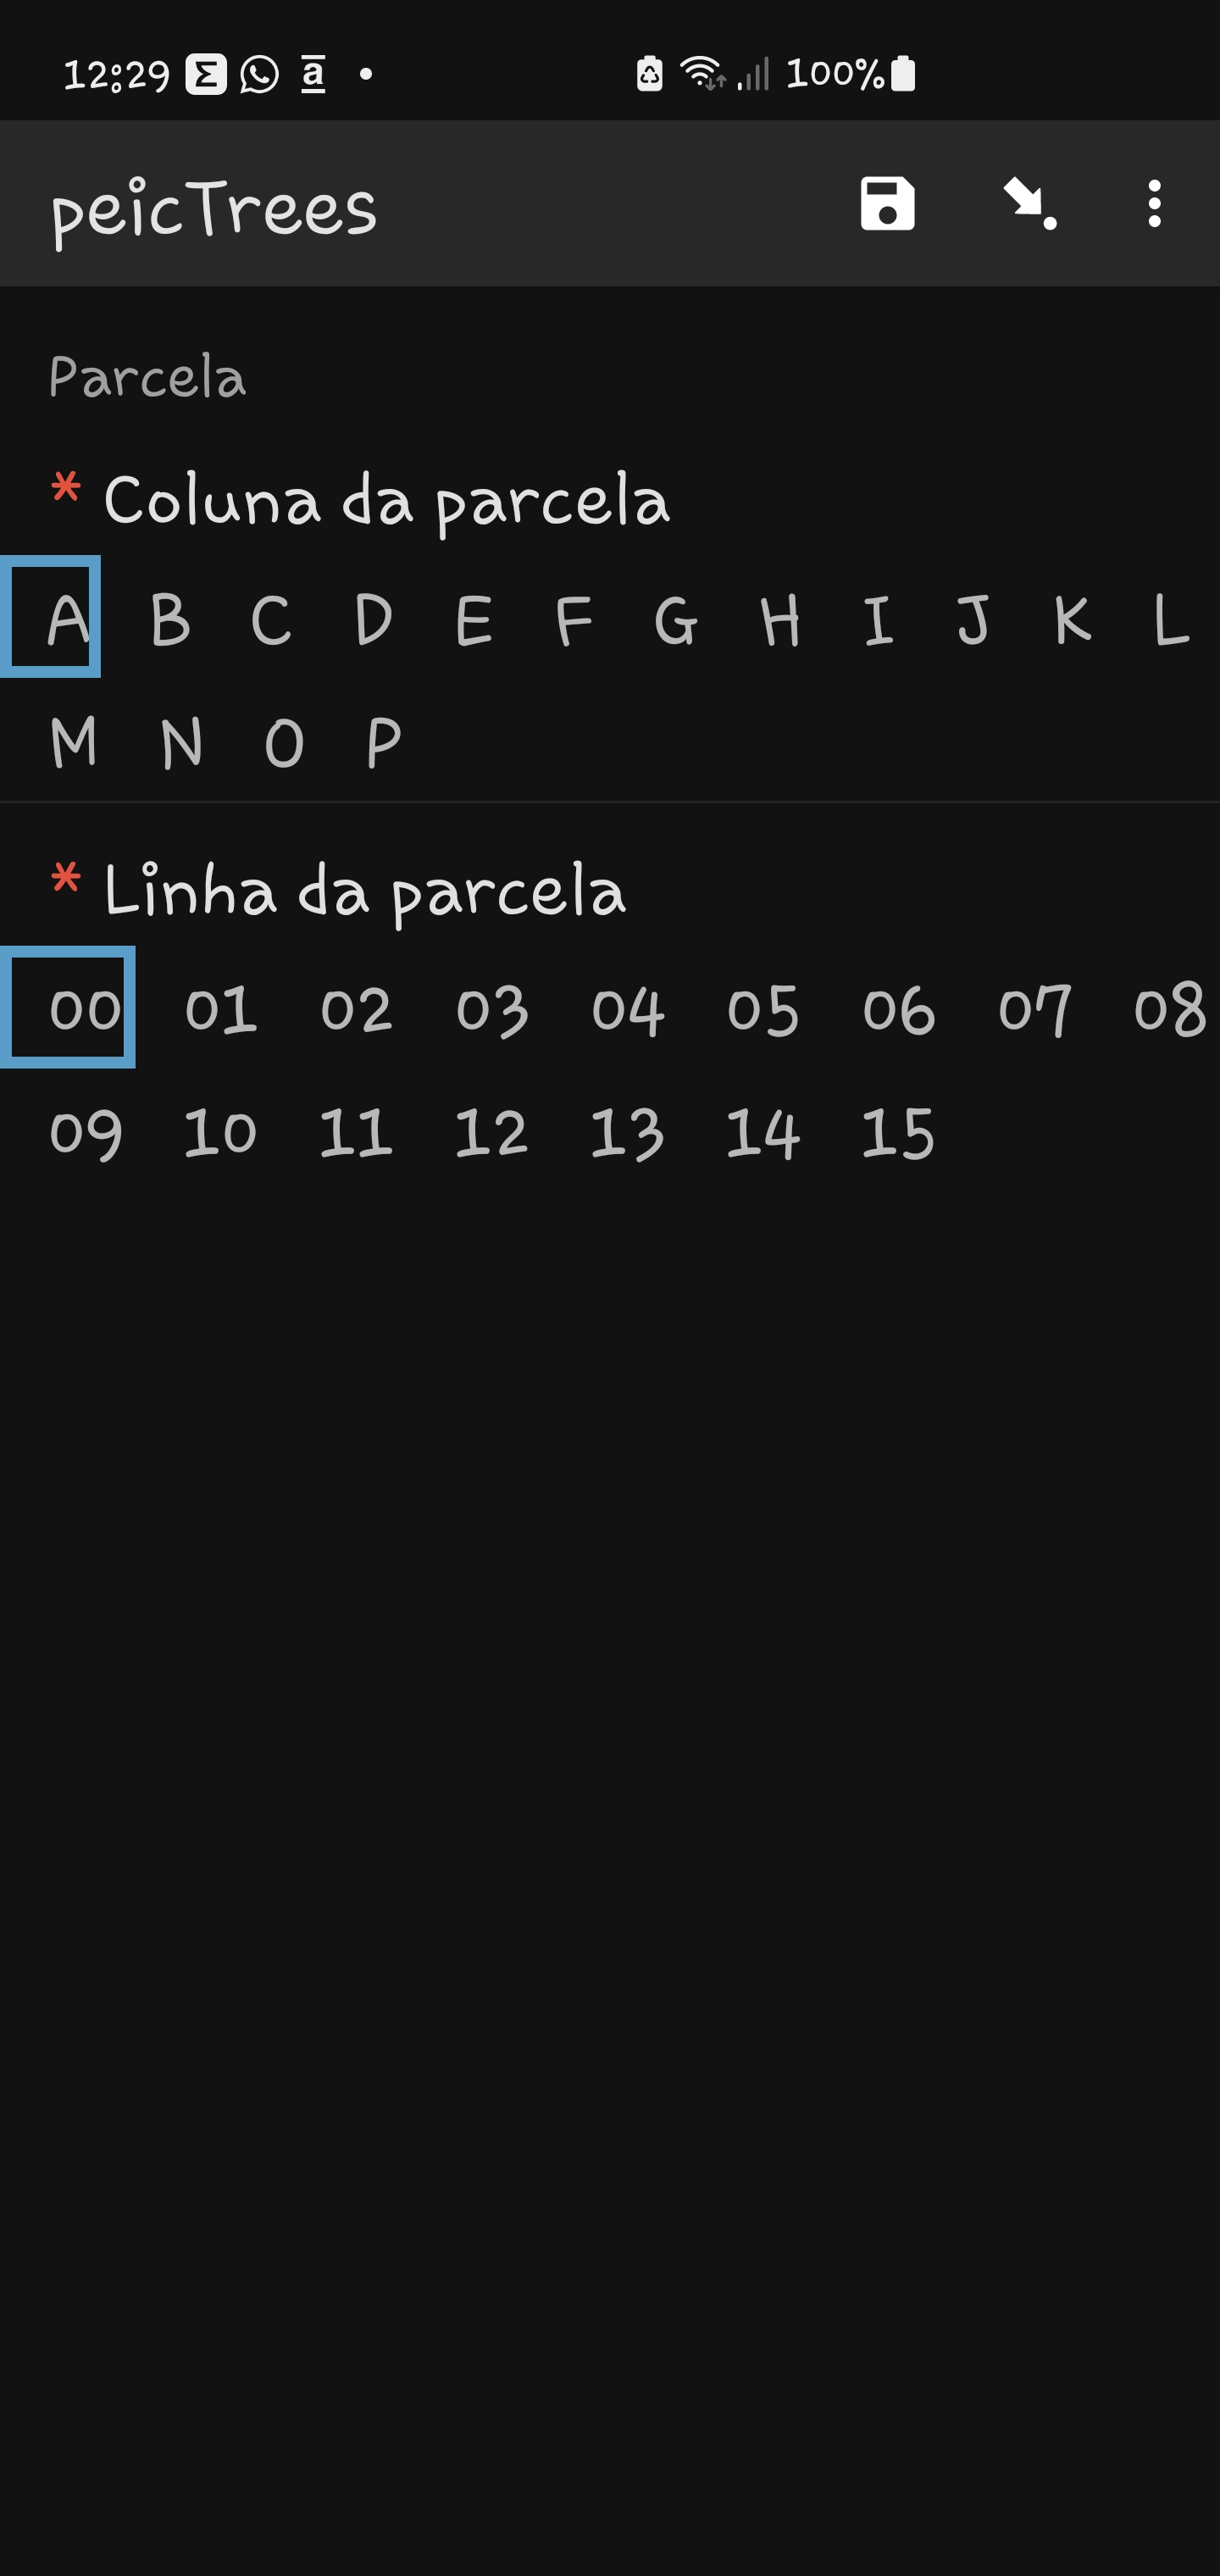
\includegraphics[width=0.5\textwidth]{media/odkSelectQuad.jpg}
  \caption{ Selecione a opção de linha (x) e coluna (y) da subparcela.}

\end{figure}


\subsection{\texorpdfstring{Árvores}{Arvores}}
\label{sec:arvores}


O próximo passo é selecionar a árvore dentro da subparcela escolhida. A próxima tela irá mostrar o mapa das árvores com diâmetro do tronco a áltura do peito (DAP) maior que 50 mm em cinza e as árvores com DAP $>$ 100mm em verde. Para selecionar pode ser necessário ampliar o mapa, utilizado o gesto usual de afastar o polegar do indicador. O círculo que representa a árvores selecionada no mapa irá mudar de cor (vermelho) e o código da espécie e o número da placa irão aparecer abaixo do mapa. O numeral ``.1'' ao final é apenas uma necessidade para que o aplicativo possa fazer a seleção, desconsidere.

\begin{figure}
  \centering
  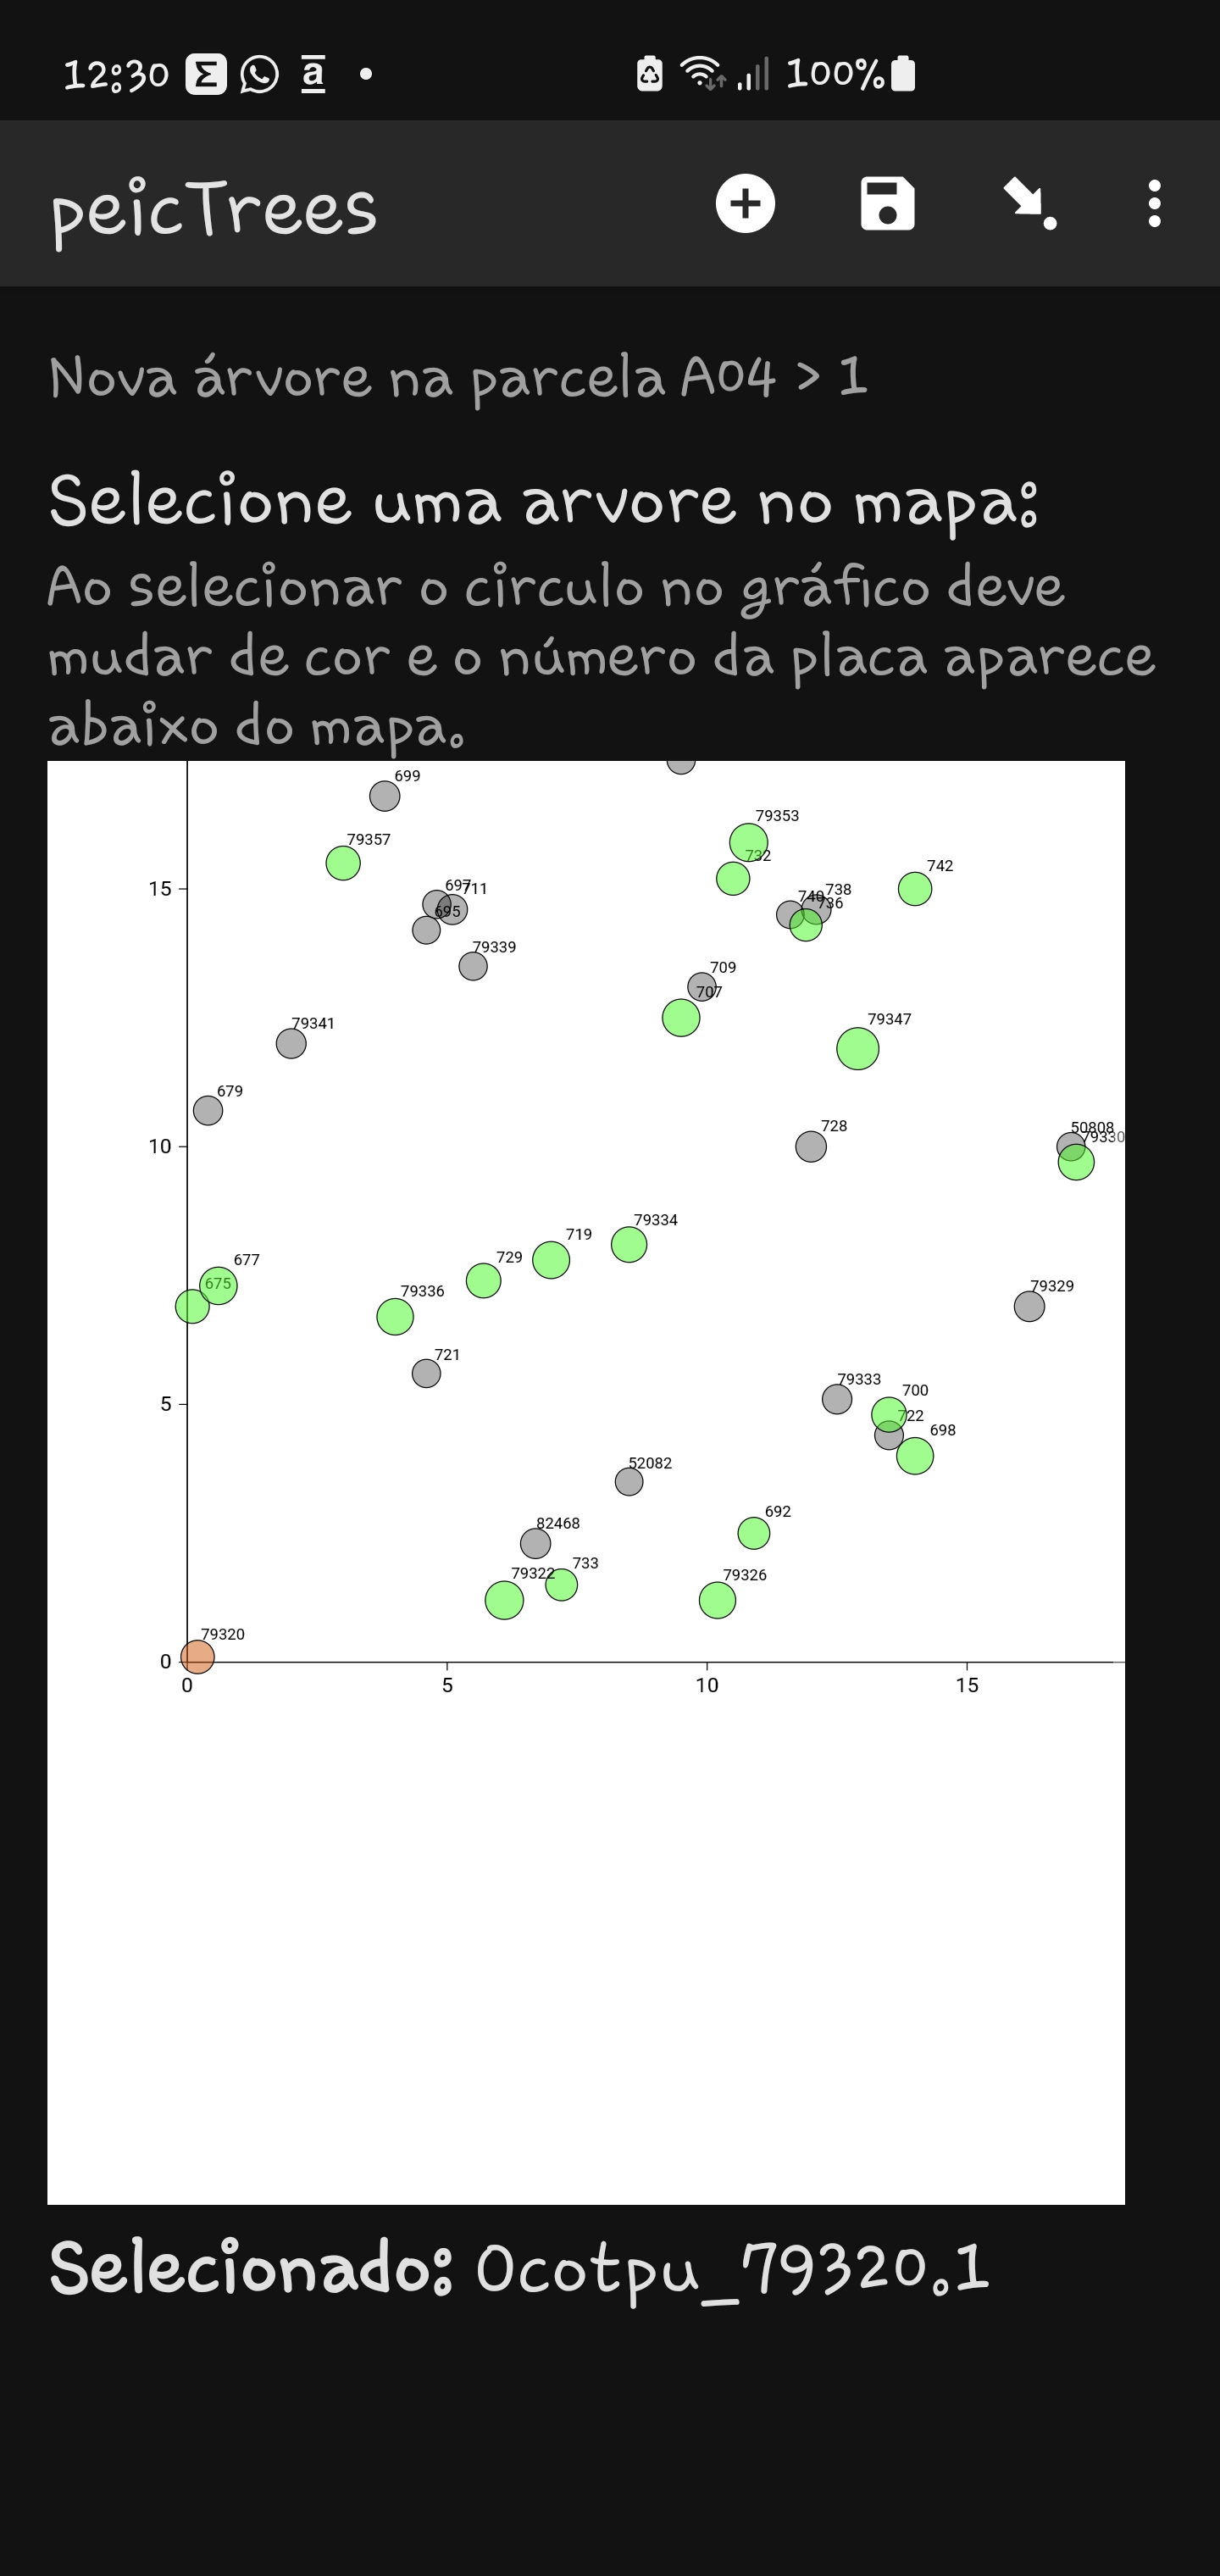
\includegraphics[width=0.5\textwidth]{media/odkSelectTree.jpg}
  \caption{ Selecione um cículos que representam as árvores na subparcela. A árvores selecionada irá ficar vermelha e o código dela aparecerá abaixo do mapa.}

\end{figure}


Siga para a póxima página fazendo o gesto com o indicador da esquerda para a direita \textbf{fora da área da figura do mapa da subparcela}.

A próxima página irá mostrar os dados da árvore selecionada.


\subsubsection{\texorpdfstring{Coordenada Geográficas -  GPS}{Coordenada GPS}}
\label{sec:coordenada_gps}


Nesse ponto é possível coletar o ponto de GPS, caso seu dispositivo tenha essa funcionalidade. Para isso é preciso selecionar \textbf{Iniciar GeoPoint}. A precisão máxia foi definida como 4m. Para alcançar essa definição o dispositivo pode demorar, a qualquer momento é possível cancelar ou salvar as coordenadas geográficas com a precisão possível no momento.   

\begin{figure}
  \centering
  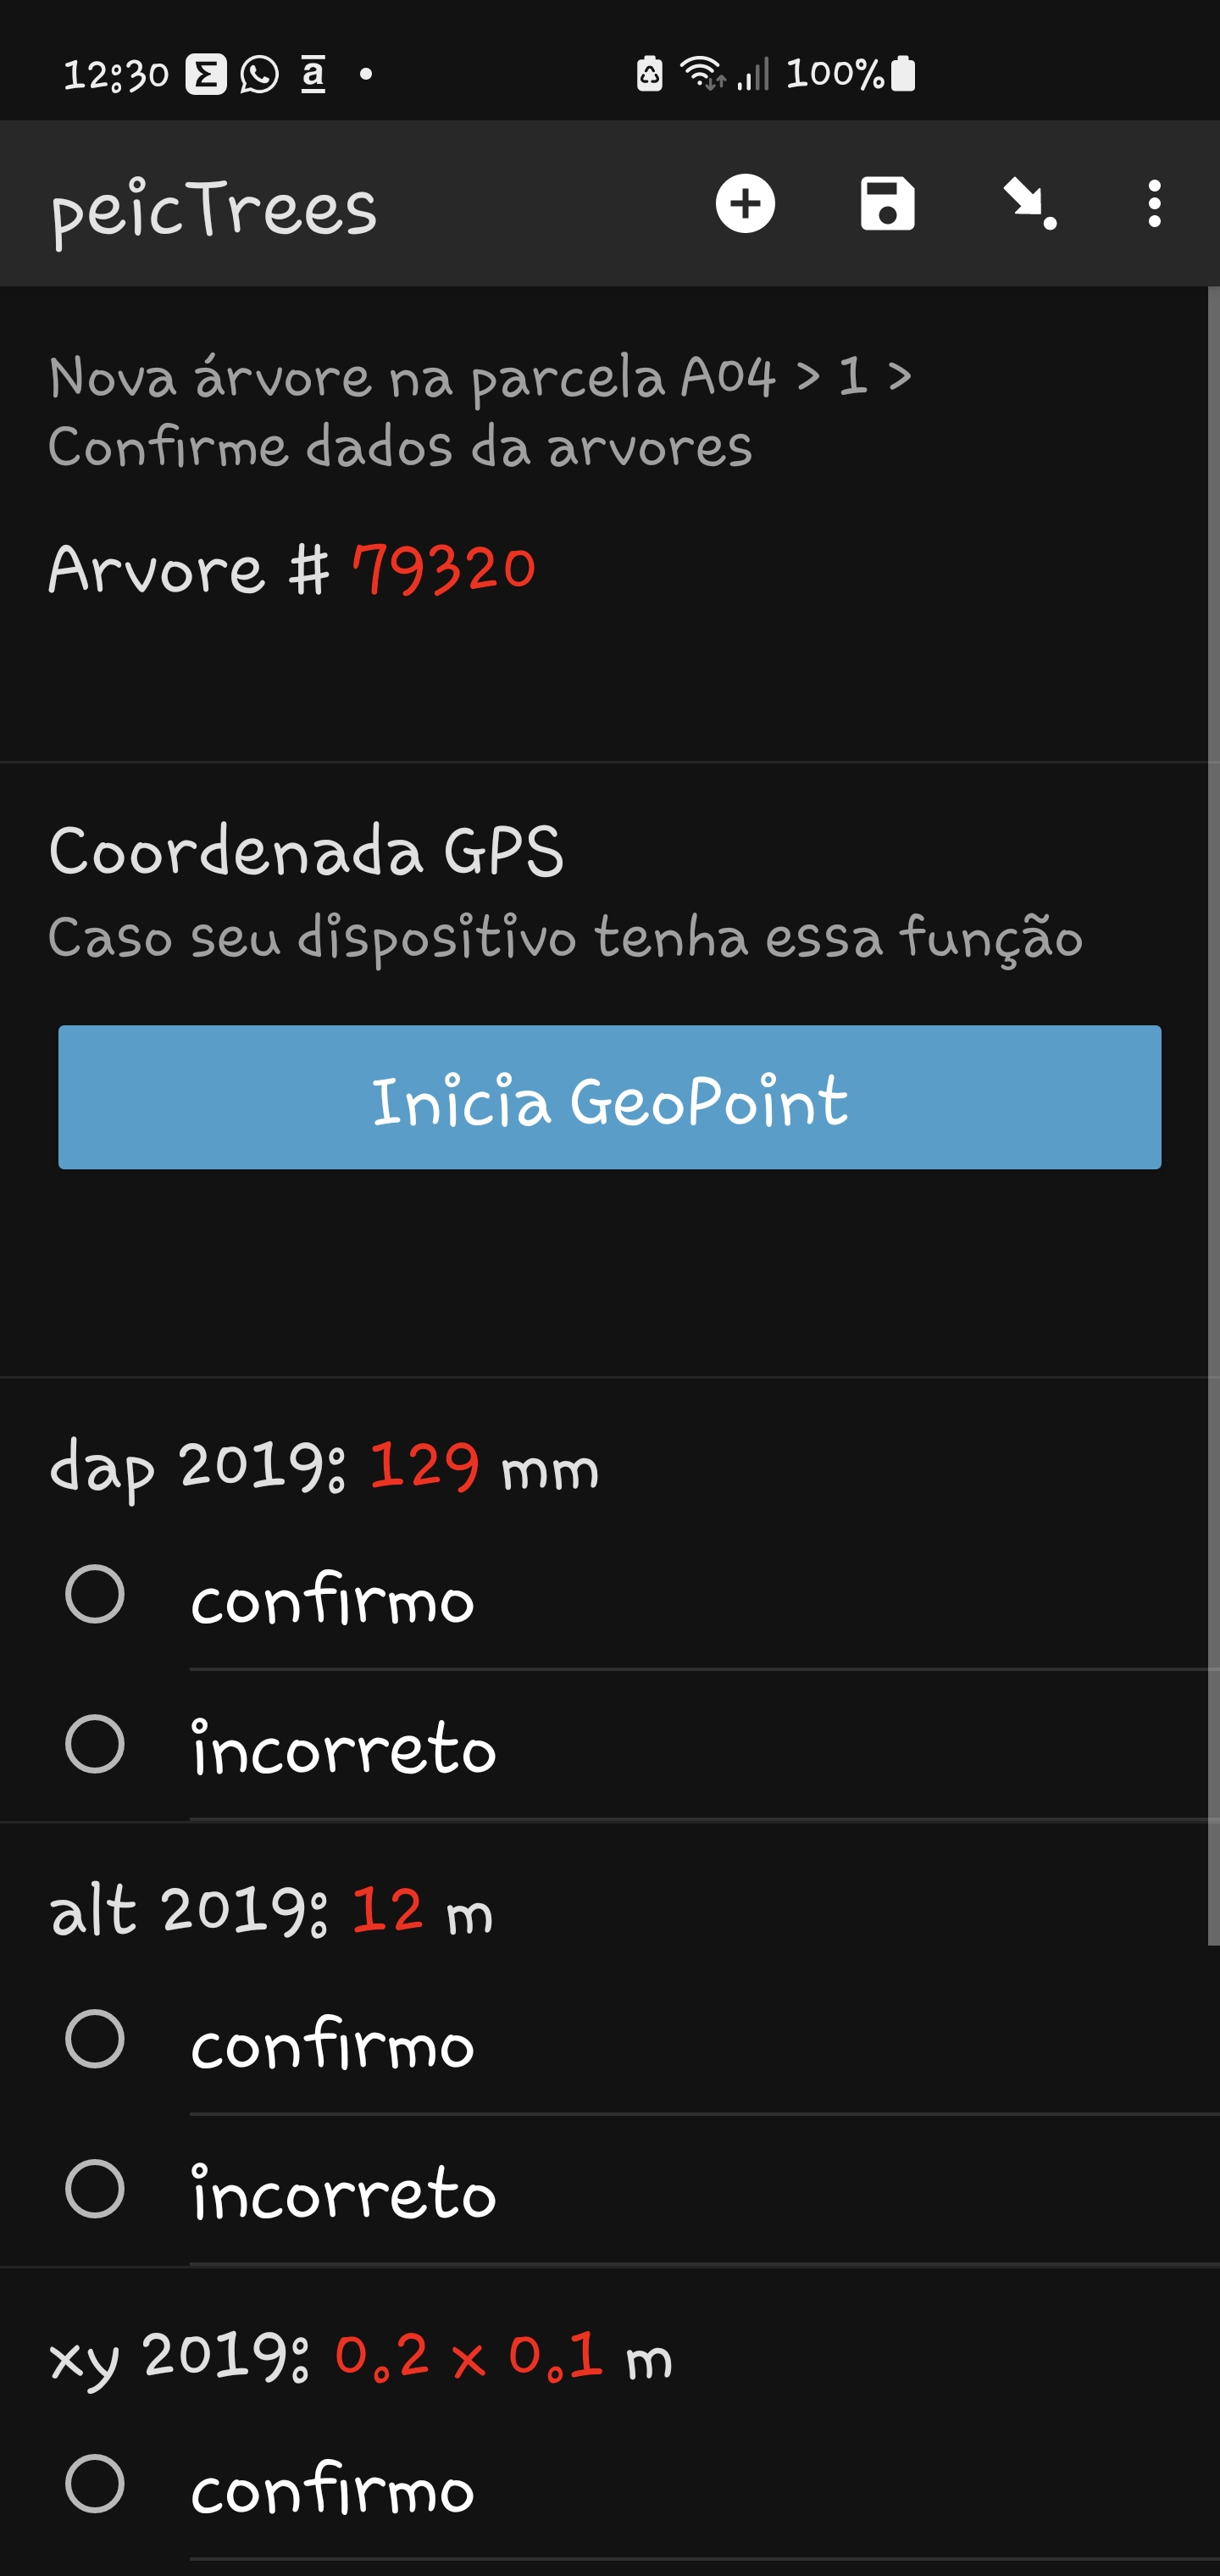
\includegraphics[width=0.5\textwidth]{media/odkSelectGPS.jpg}
  \caption{Inicie a leitura das coordenadas geográficas selecionando \textbf{Iniciar GeoPoint}.}

\end{figure}


\subsubsection{\texorpdfstring{Confirma dados}{Confirma dados}}
\label{sec:arvores}


Nesse ponto pedimos que confirme os dados da árvore. Isso não é mandatório, mas caso queira contribuir para a estimativa de erros da parcela, pode confirmar ou não as informações.


\subsection{\texorpdfstring{Foto da Árvore}{Foto da Arvore}}
\label{sec:arvores}


A próxima tela pergunta se quer tirar uma foto da árvore, selecione \textbf{sim} para abrir a câmera do disposito e associar uma foto à árvores selecionada.

Em seguida aparece as opções de tipo de foto que será tomada. Selecione uma das opções ou inclua outra na opção correspondente. 

\begin{figure}
  \centering
  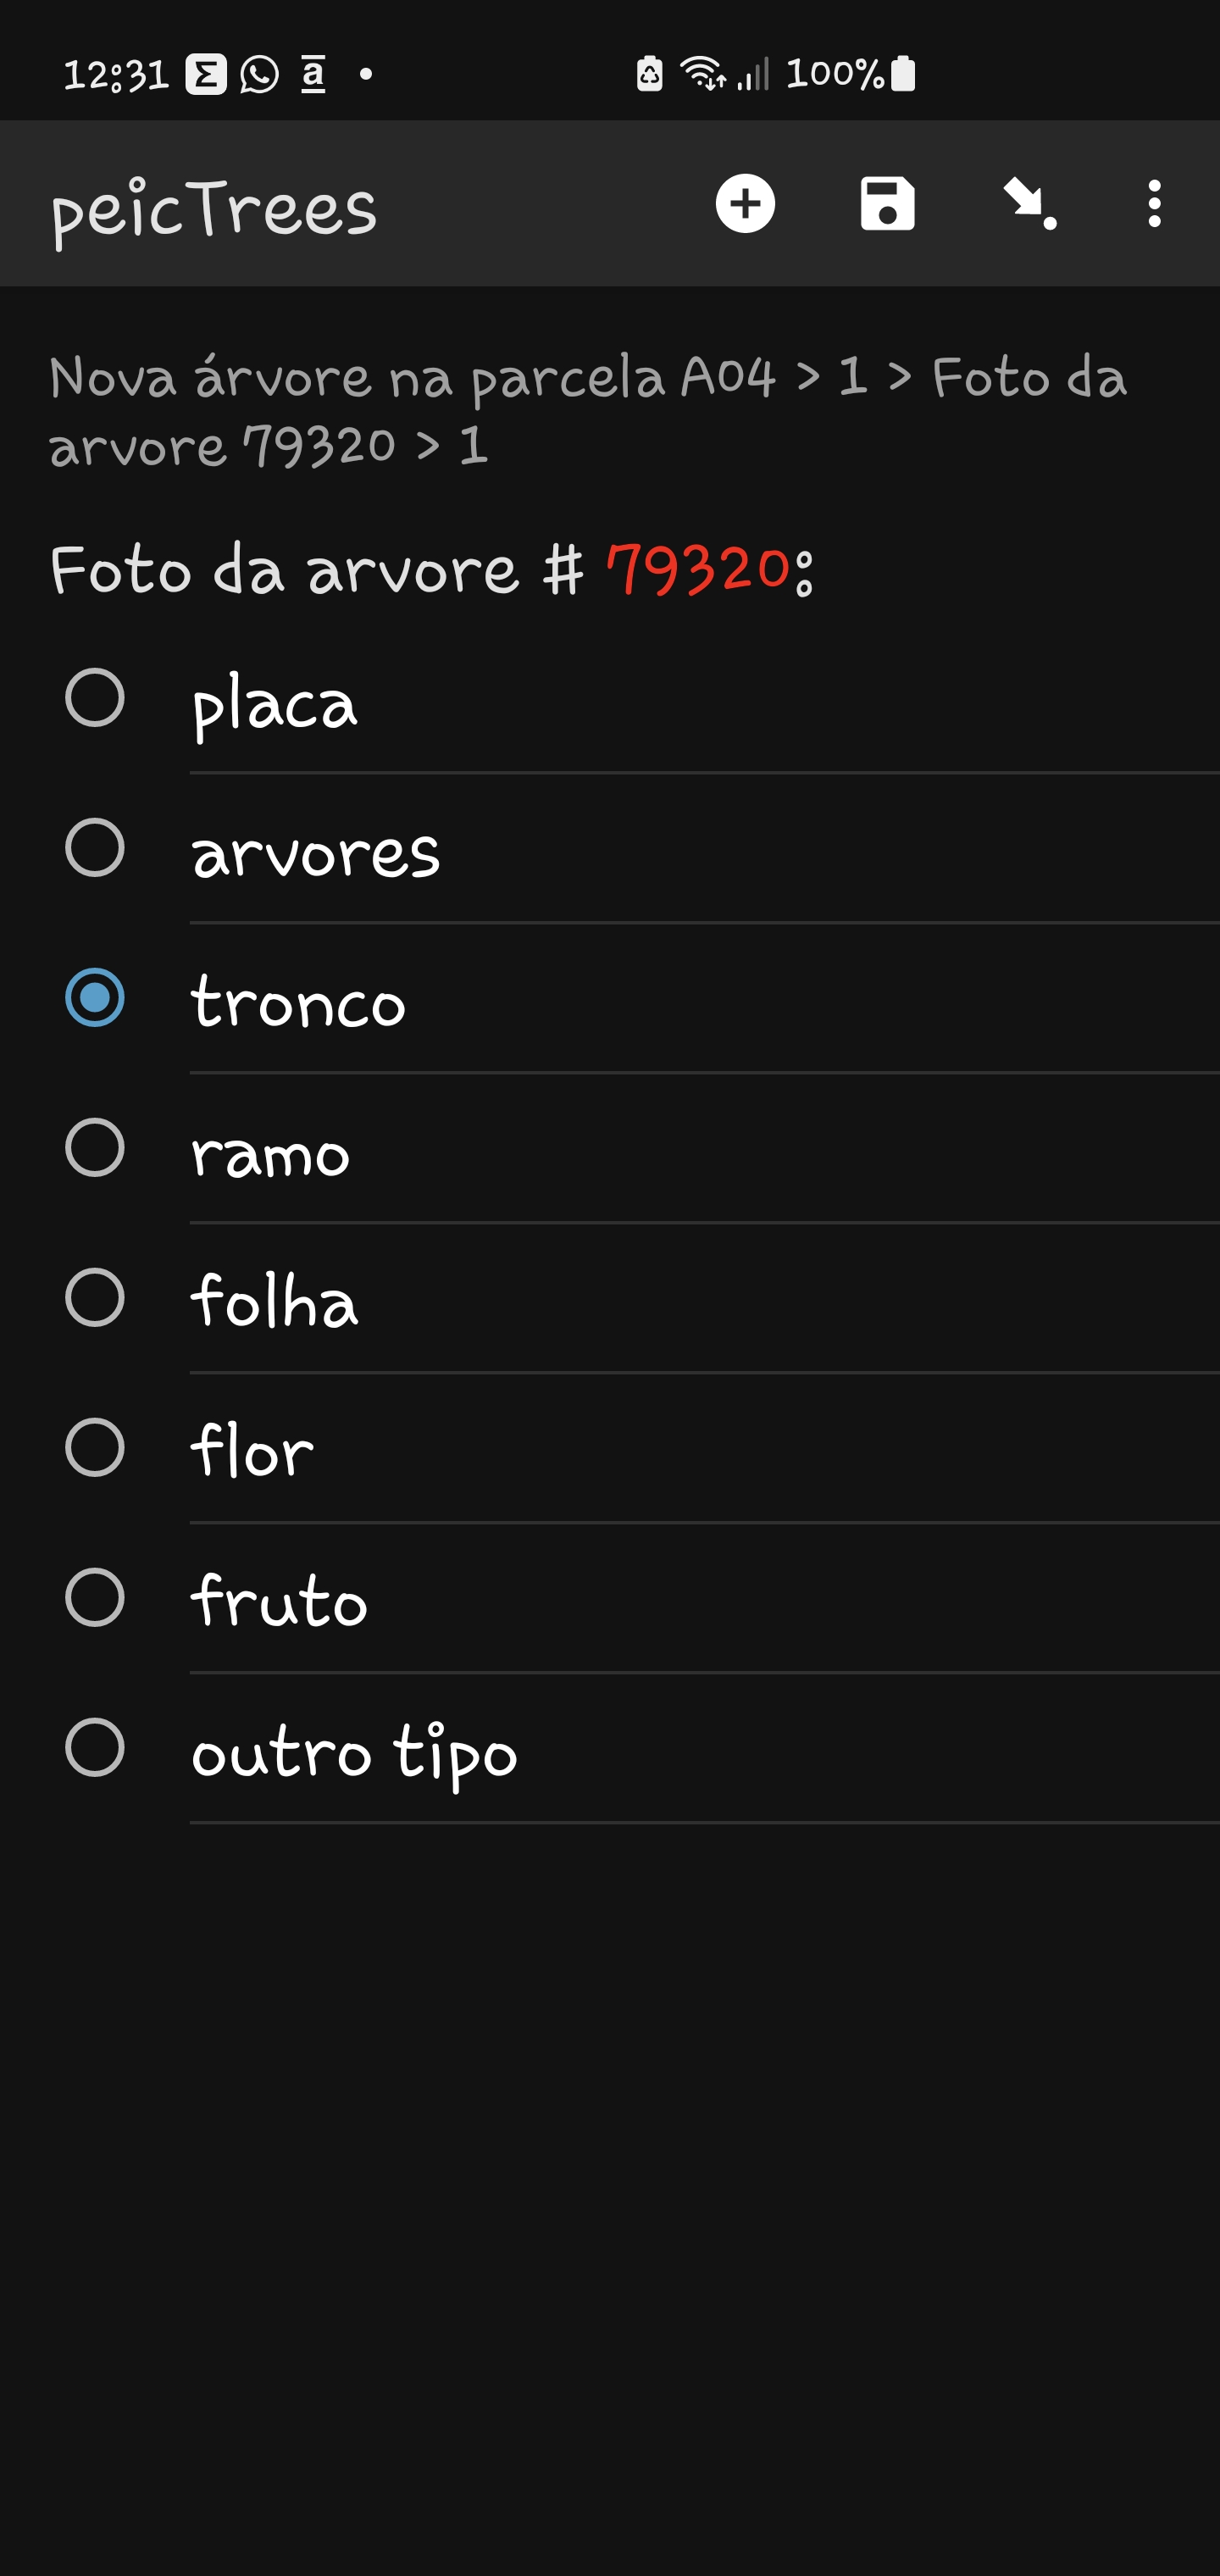
\includegraphics[width=0.5\textwidth]{media/odkSelectFotoType.jpg}
  \caption{ Selecione o tipo de foto que será tomada.}
\end{figure}



Ao finalizar a tomada do foto, o aplicativo irá perguntar se quer incluir outra para a mesma árvore, caso contrário irá perguntar se quer selecionar outra  árvores  na mesma parcela.



\begin{center}
\begin{figure}
\centering  
\begin{subfigure}{.4\textwidth}
  %\centering
  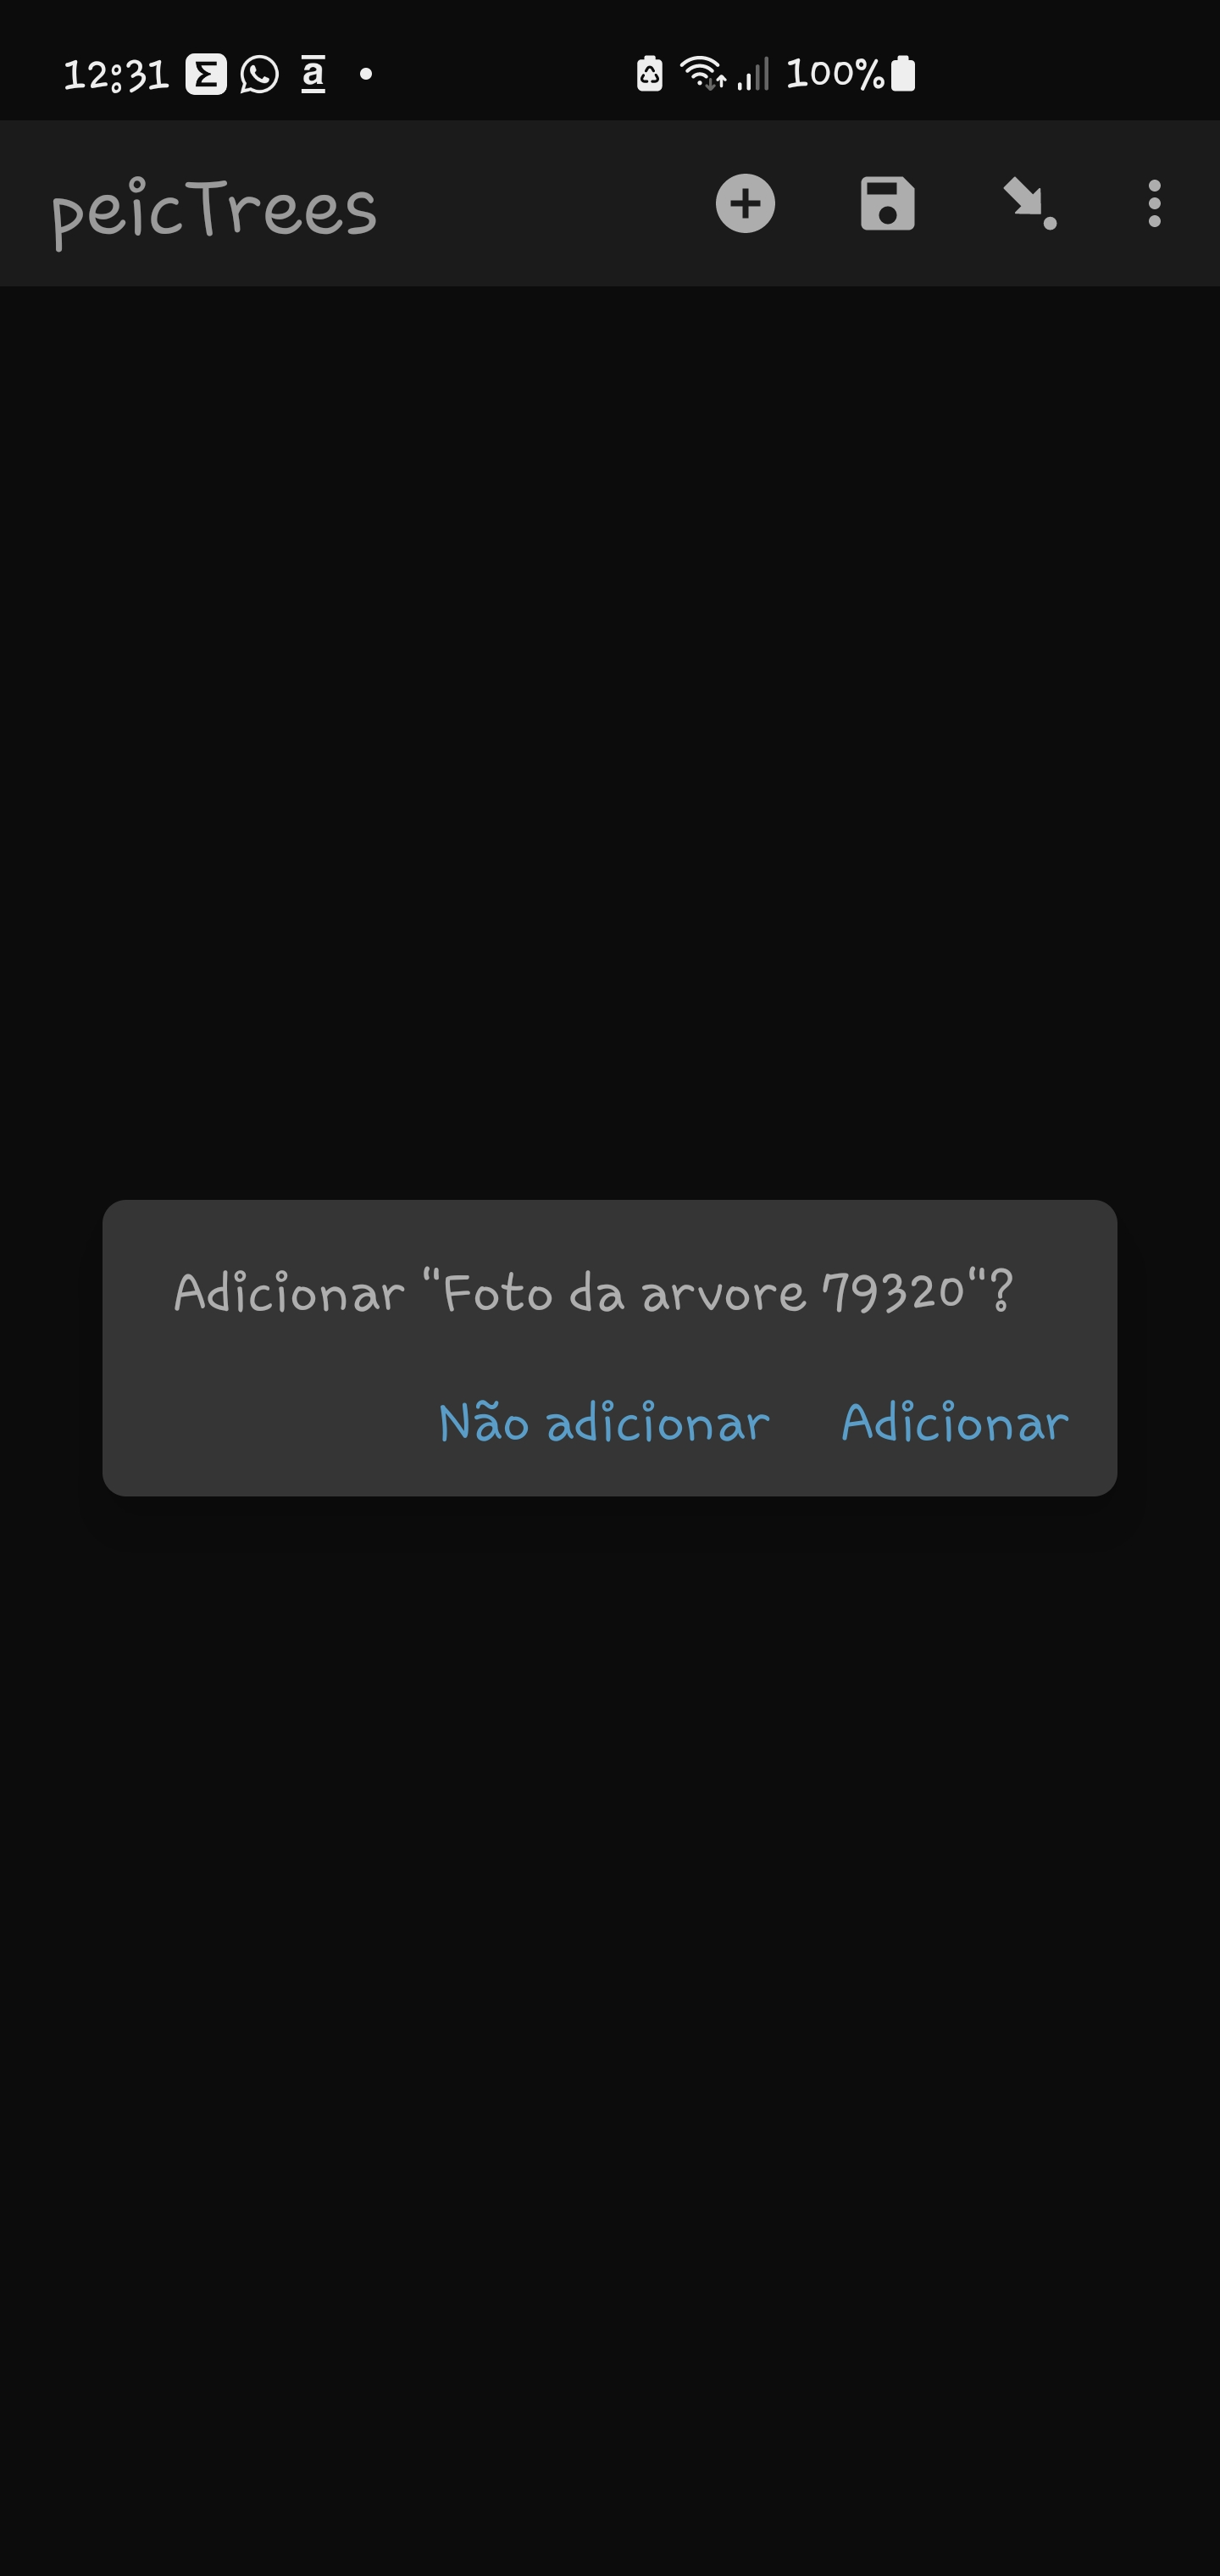
\includegraphics[width=.9\linewidth]{media/odkSelectNewFoto.jpg}
  %% \caption{Tela de selecão de nomes da equipe}
  %% \label{fig:app1}
\end{subfigure}\hfil
\begin{subfigure}{.4\textwidth}
  %\centering
  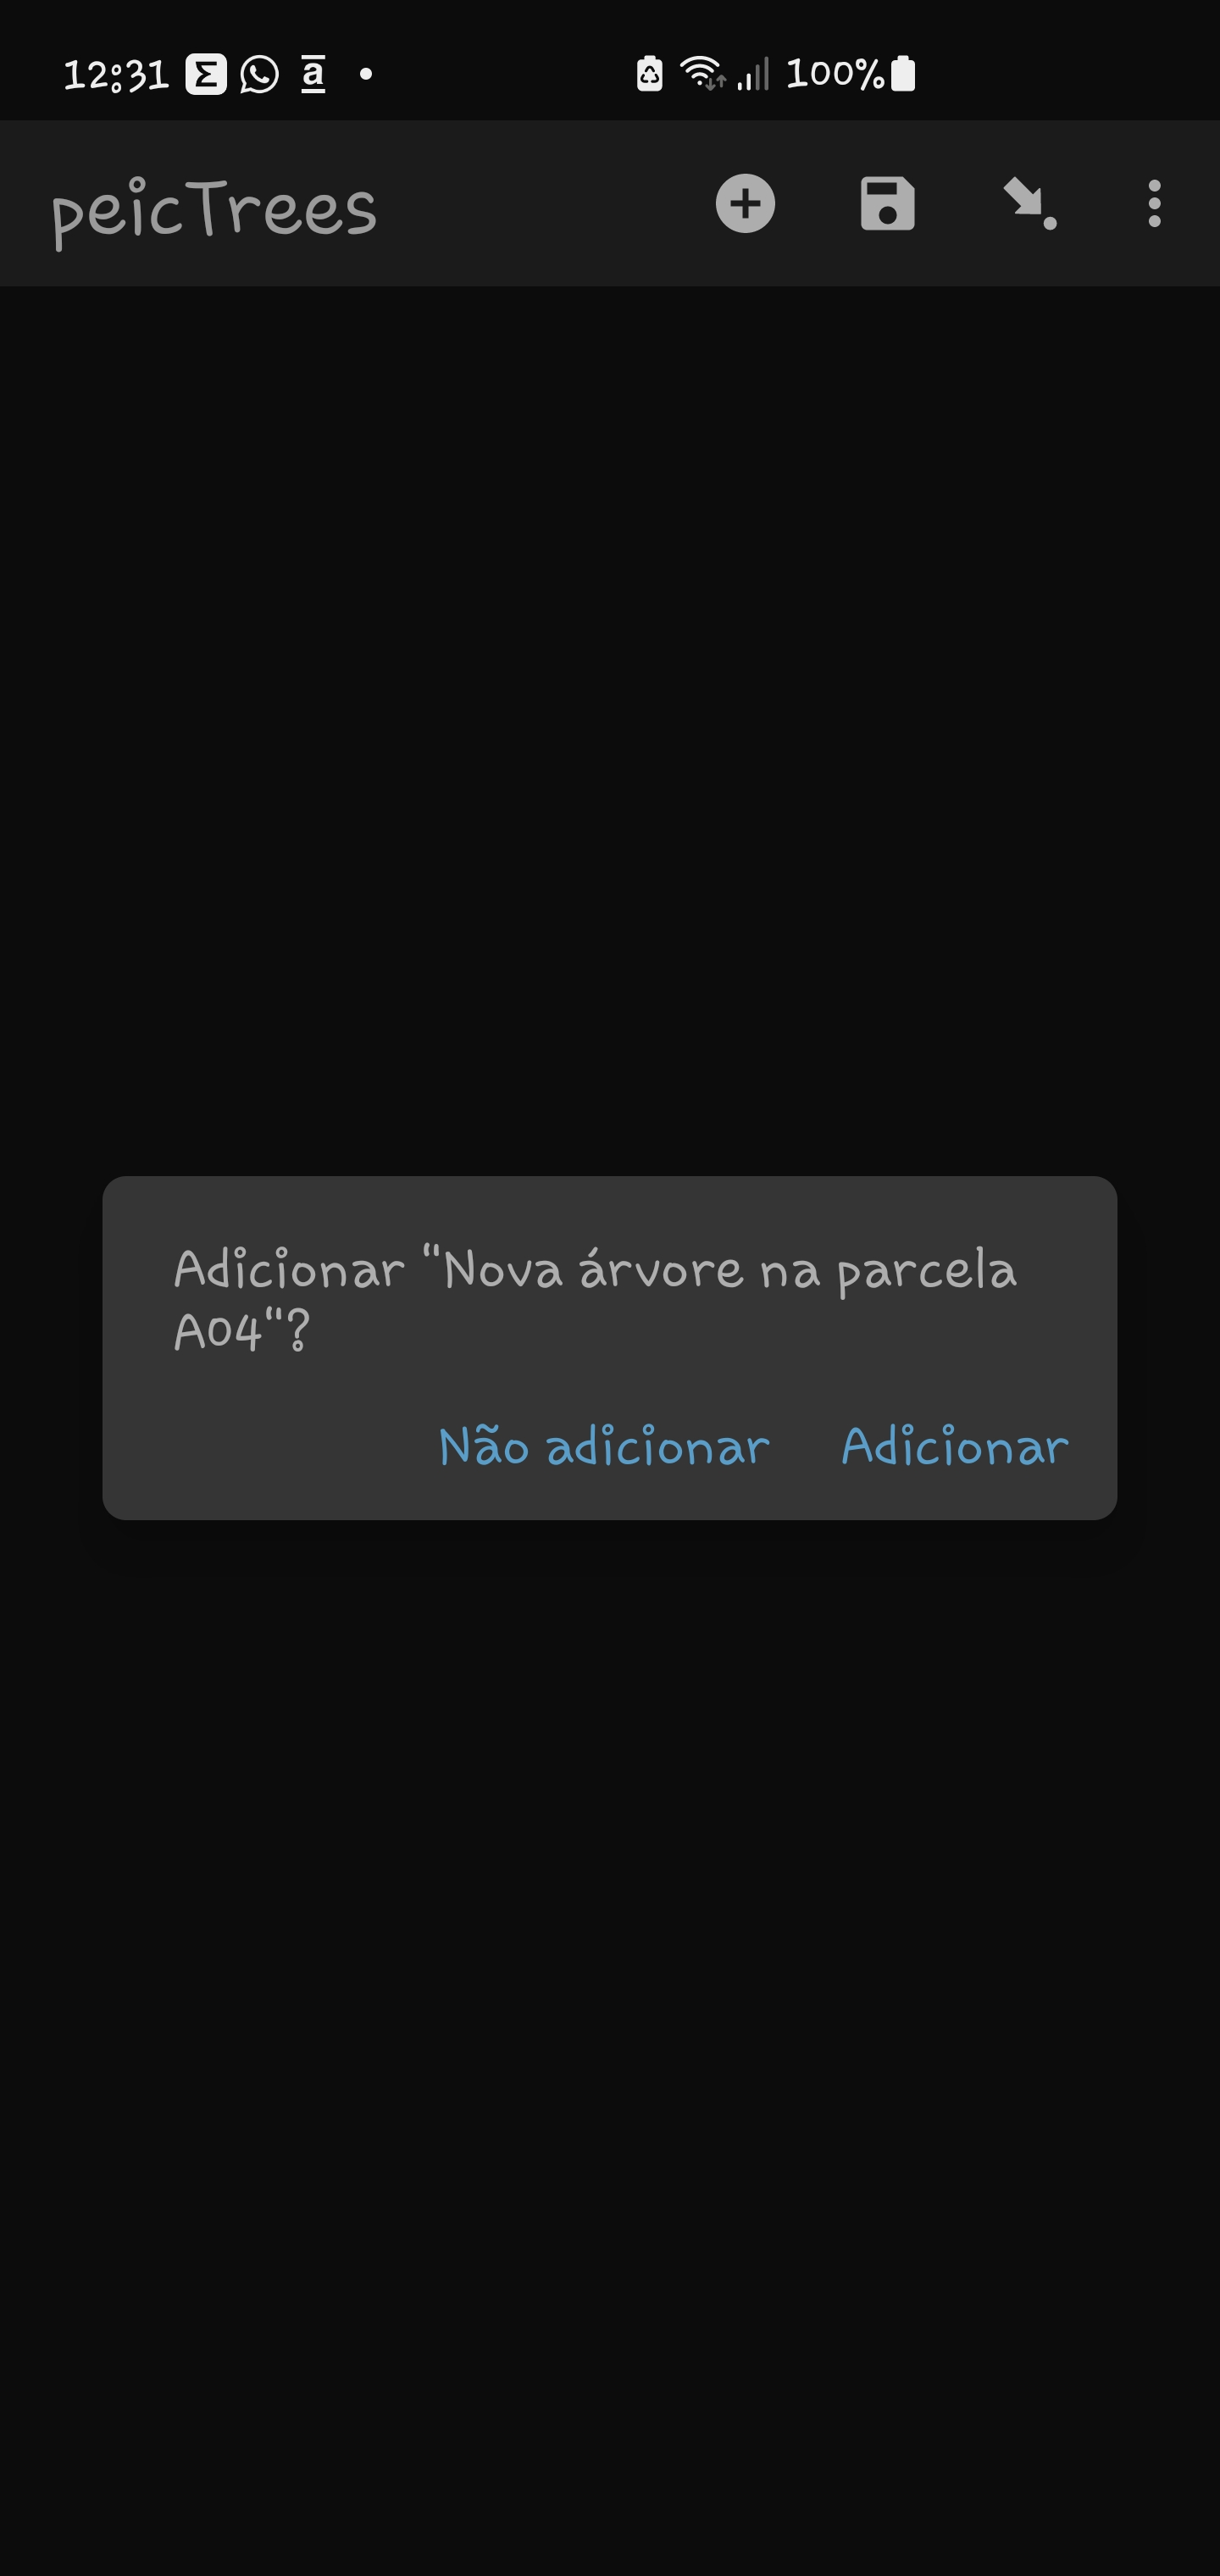
\includegraphics[width=.9\linewidth]{media/odkSelectNewTree.jpg}
  %% \caption{Tela de seleção da parcela de 20x20 m}
  %% \label{fig:app2}
\end{subfigure}\hfil

\caption{Telas onde é possível adicionar nova foto para a mesma árvore (esquerda) e selecionar outra árvore na mesma subparcela (direita) no \textbf{ODKCollect - peicTrees}}
\label{fig:app}
\end{figure}
\end{center}




\subsection{Salvando os dados}
\label{sec:salva}


Caso selecione \textbf{Não adicionar} nova árvore o aplicativo abrirá a página para salvar os dados. Marque o formulário como finalizado e selecione \textbf{Salvar Formulário e Sair}  


Caso precise de alguma ajuda procure o Alexandre ou um de seus alunos, Marcel e Luisa, que estão em trabalho de campo na parcela nesta mesma excrusão.



\end{document}
 equipe deve, ao final da atividade, salvar a pasta \textbf{\underline{odk}} com todas as subpastas, e encaminhar para os professores.
